\documentclass[12pt]{article}
\usepackage[a4paper, margin=1in]{geometry}
\usepackage{graphicx}
\usepackage{caption}
\usepackage{float}
\usepackage{booktabs}
\usepackage{lipsum}
\usepackage{setspace}
\usepackage{parskip}
\def\gitcommit{a5ac882}
\def\builddate{2025-04-20}


\title{Task 1A: Initial Data Analysis}
\author{Sofia French}
\date{\today}

\begin{document}

\maketitle

\section*{Overview}

This document summarises the exploratory data analysis (EDA) and visualisation steps completed on \today for the Vinho Verde wine dataset. The focus has been on understanding how perceived wine quality varies between red and white varieties, through data analysis: specifically, distribution plots.

\section*{Quality Distribution – Red Wine}

The first analysis targeted the distribution of the \texttt{quality} variable in the red wine dataset. The quality values range from 3 to 8, with most samples concentrated around 5 and 6.

\begin{figure}[H]
    \centering
    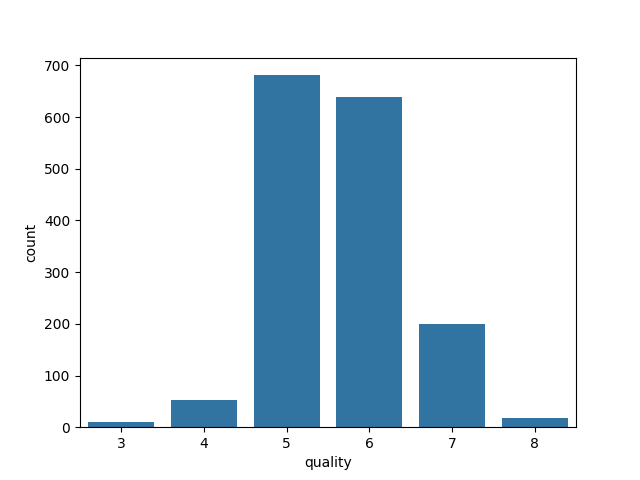
\includegraphics[width=0.75\textwidth]{../figures/red_wine_quality.png}
    \caption{Distribution of Quality Scores in Red Wine Dataset}
    \label{fig:red_quality}
\end{figure}

\textbf{Observation:} The majority of red wine samples are rated as quality 5 and 6, which together make up the bulk of the dataset. There is a sharp drop for higher quality scores (7 and 8), and very few samples with scores below 4.

\section*{Quality Distribution – White Wine}

The same analysis was performed on the white wine dataset.

\begin{figure}[H]
    \centering
    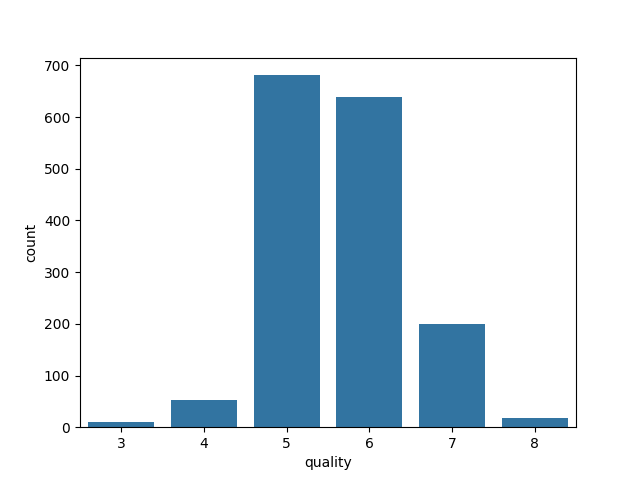
\includegraphics[width=0.75\textwidth]{../figures/white_wine_quality.png}
    \caption{Distribution of Quality Scores in White Wine Dataset}
    \label{fig:white_quality}
\end{figure}

\textbf{Observation:} Like red wines, most white wines fall into the 5–6 quality range. However, white wines show a broader spread — with more wines rated as 7 and 8 compared to red. There's also a noticeable number of white wines rated as 4, which wasn't as prominent in the red wine data.

\section*{Red vs. White Comparison}

For a side-by-side comparison, both quality distributions were plotted on a single figure.

\begin{figure}[H]
    \centering
    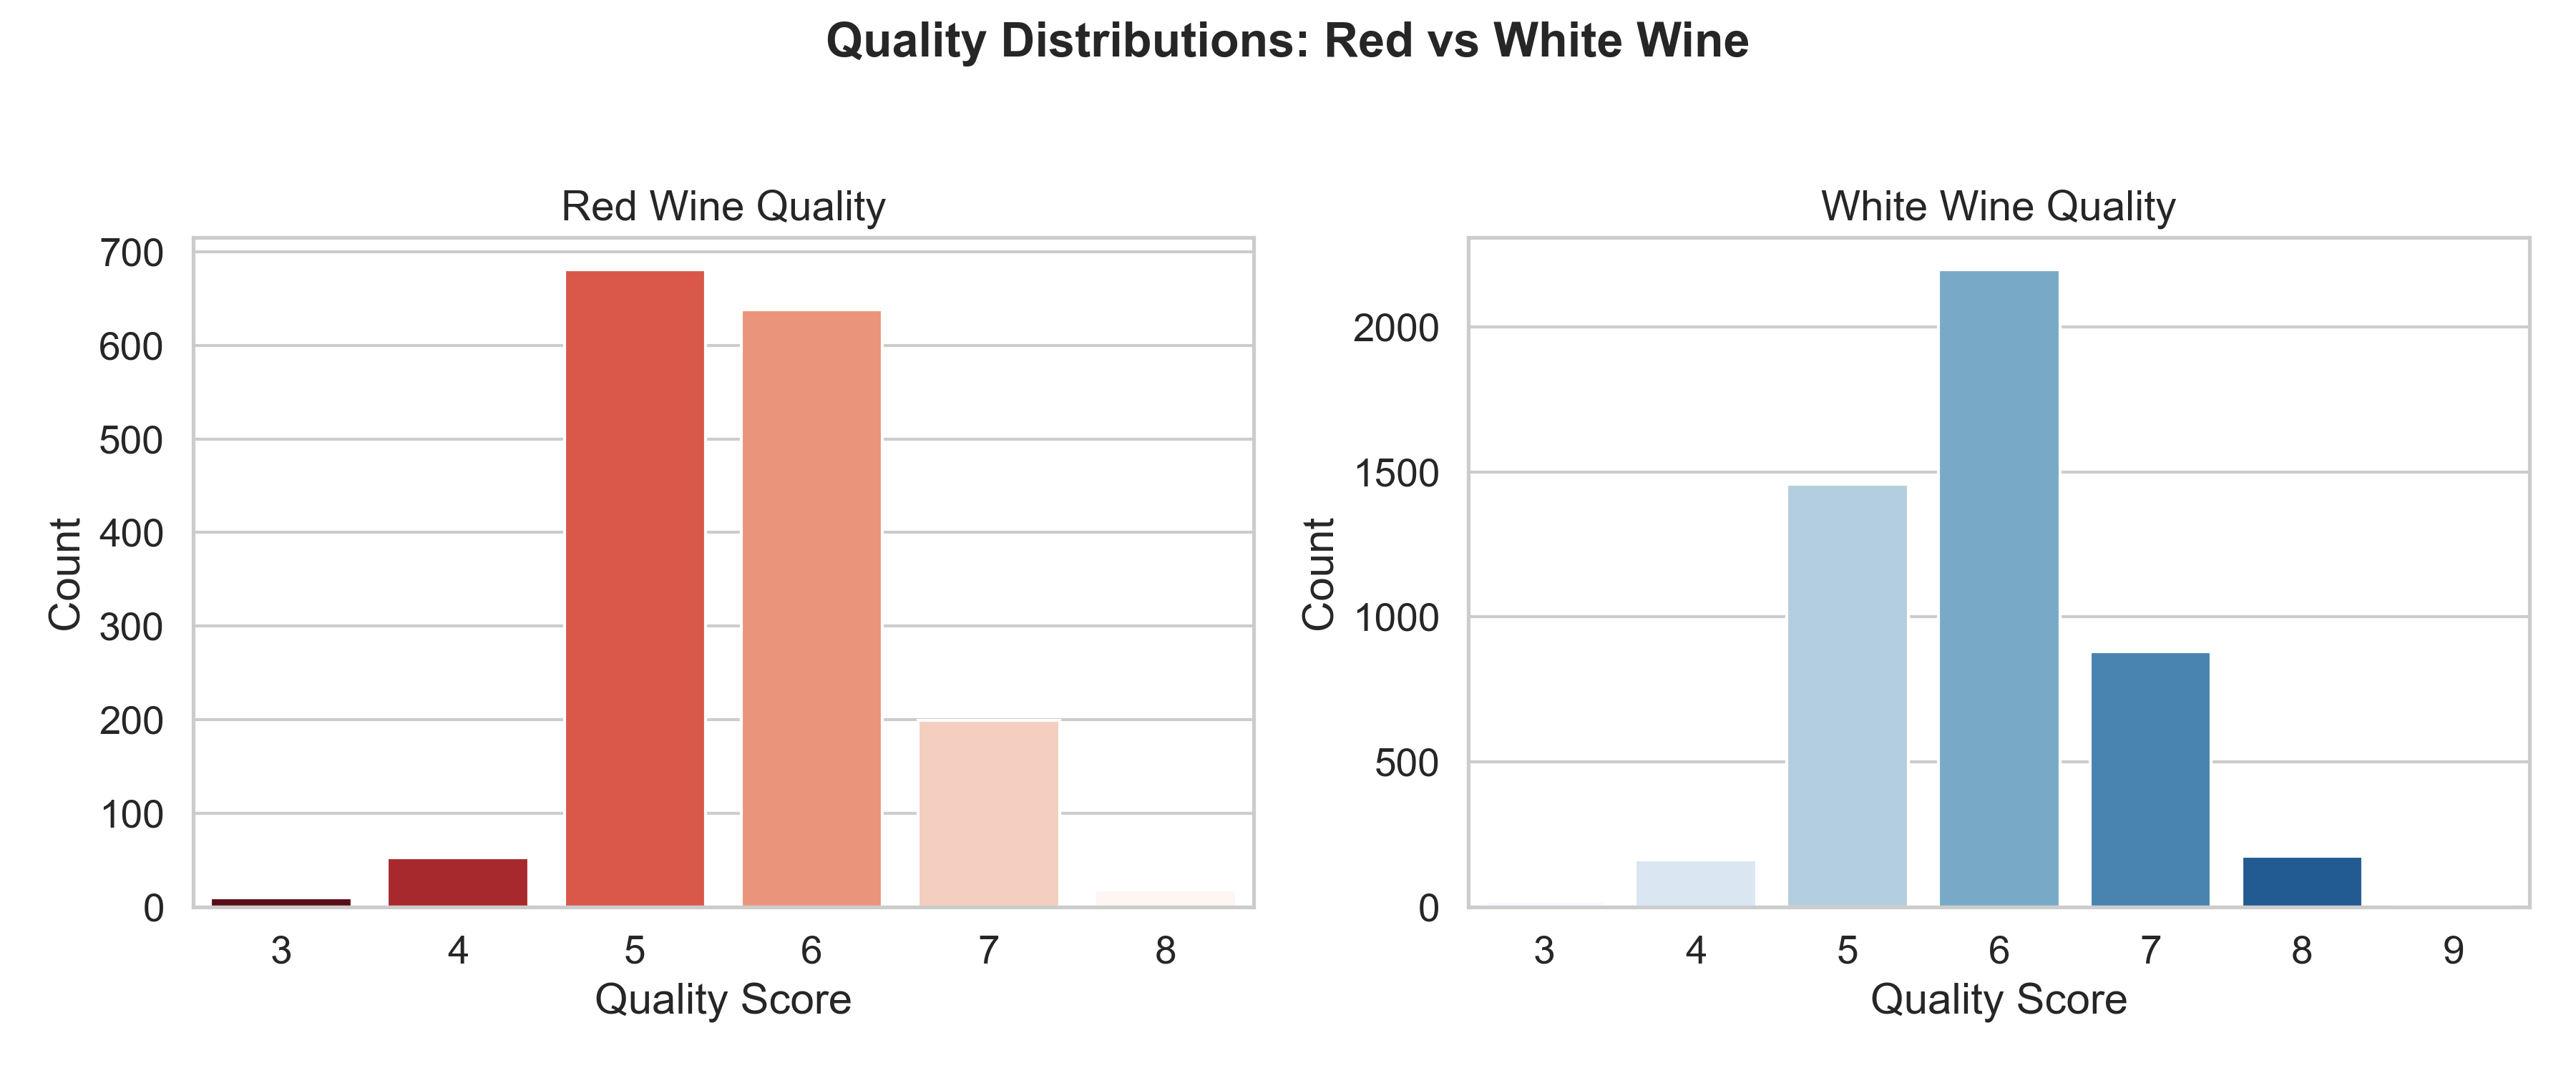
\includegraphics[width=\textwidth]{../figures/wine_quality_comparison.png}
    \caption{Side-by-Side Distribution of Red and White Wine Quality}
    \label{fig:combined_quality}
\end{figure}

\textbf{Insights:}
\begin{itemize}
    \item Red wine quality is tightly clustered around 5 and 6.
    \item White wine quality is more variable, with a longer right tail (which suggests more high-quality samples).
    \item Overall, white wine shows a slightly higher mean quality, though both distributions are skewed and non-uniform.
\end{itemize}

\section*{Next Steps}

\end{document}
